%<dscrpt>Chute d'un parachutiste et méthode d'Euler.<dscrpt>
On modèlise la chute d'un parachutiste à partir du moment où son parachute s'est ouvert en notant $v(t)$ la fonction représentant sa vitesse verticale au temps $t$ et en admettant que cette fonction vérifie
\begin{displaymath}
  v'(t) = g - K v(t)^2
\end{displaymath}
où $g$ est l'accélération de la pesanteur, $K$ une constante positive (qui dépend du parachute et de la masse du parachutiste). On note $v_0=v(0)$.\newline
On discrétise le problème entre $0$ et $T$ en utilisant des instants $t_0=0,t_1,\cdots,t_n=T$ avec un pas constant.

\begin{enumerate}
  \item Former les relations de récurrence définissant les valeurs $v_1,\cdots,v_n$ associées à la méthode d'Euler.
  \item \'Ecrire en Python une fonction \texttt{vpara(v0,T,n)} qui renvoie la liste des temps discrets et la liste des $v_i$. Les valeurs de $g$ et $K$ sont constantes: $g=9.81$ et $K= 0.0357$ (avec les unités usuelles).
  \item La figure \ref{fig:Eeulerpara_1} est le résultat de l'exécution du code suivant :
\begin{verbatim}
vini = [0.,10.,20.,30.]
for v in vini:    
  truc = vpara(v,6.5,100)
  plt.plot(truc[0],truc[1])  
\end{verbatim}
Que peut-on conjecturer?
\begin{figure}[h]
  \centering
  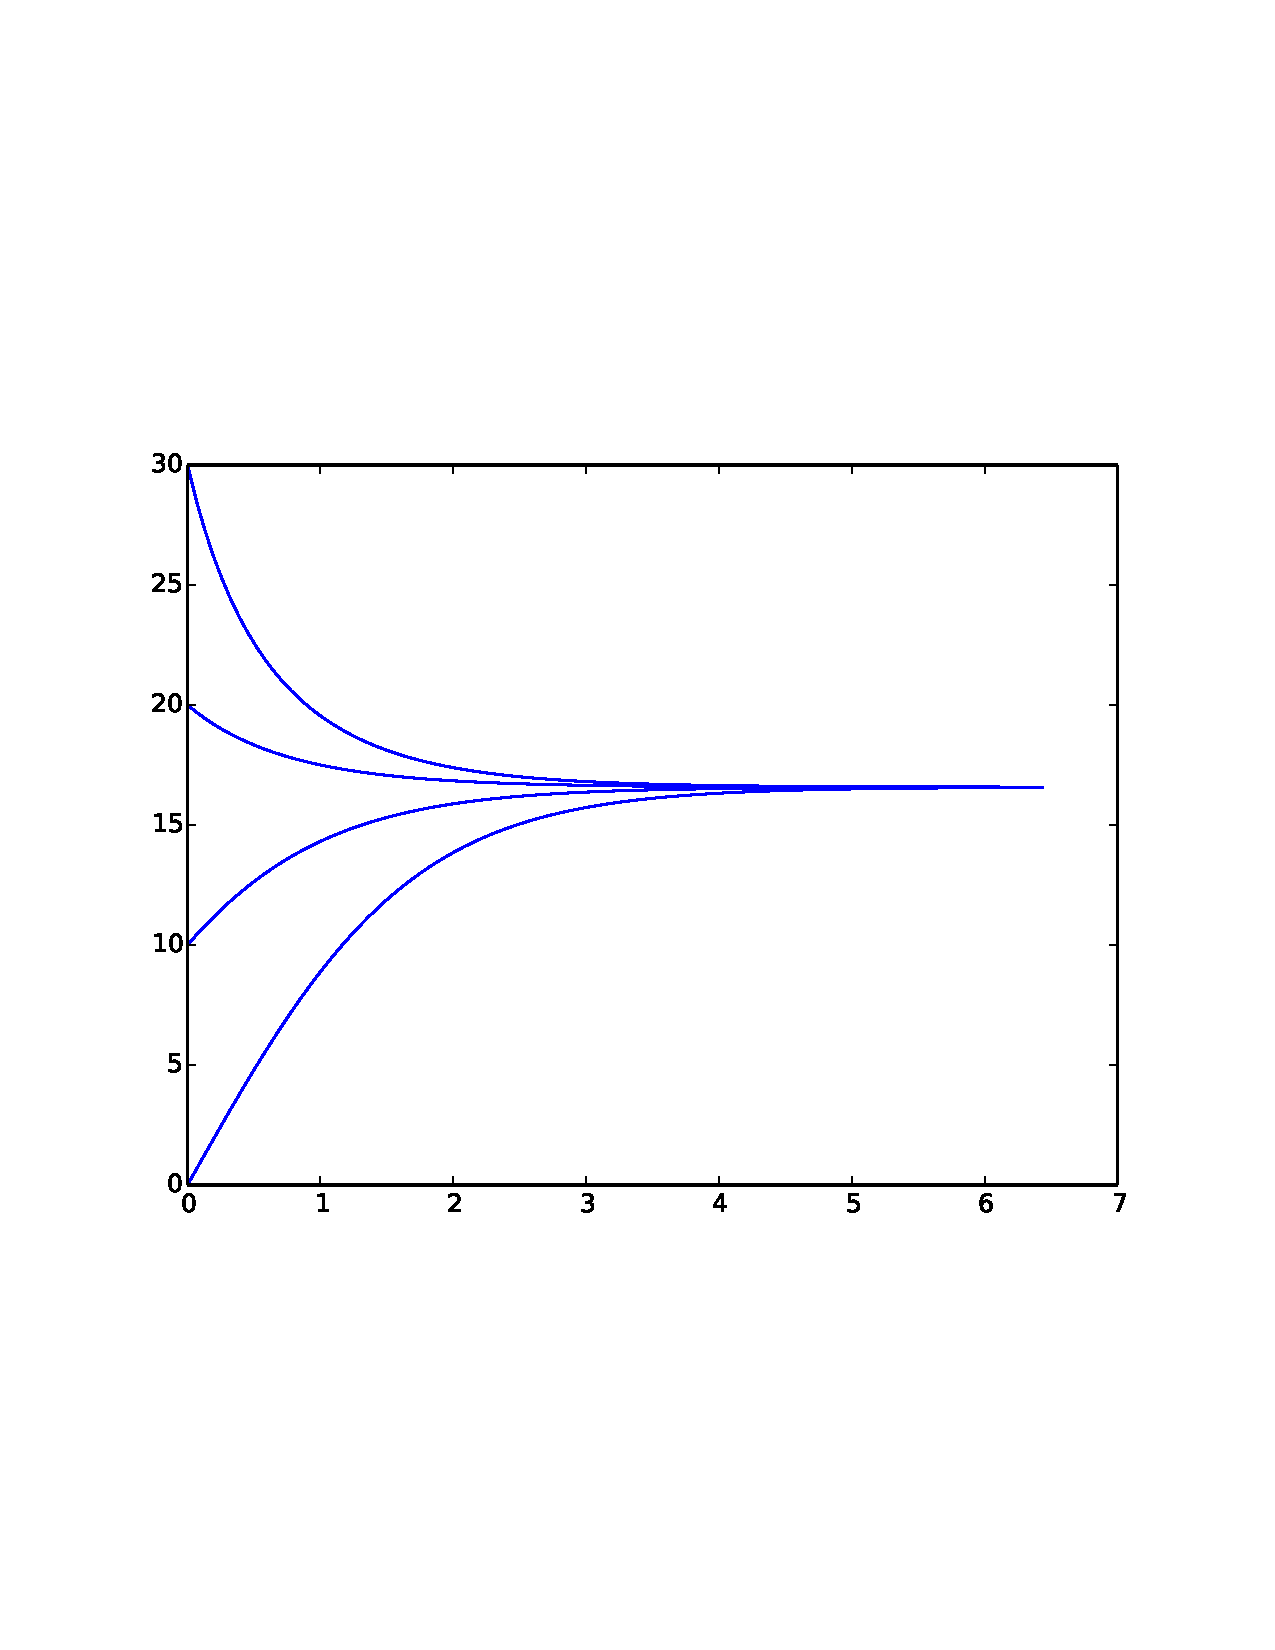
\includegraphics[width=8cm]{./Eeulerpara_1_fig.pdf}
  % Eeulerpara_1.pdf: 0x0 pixel, 0dpi, nanxnan cm, bb=
  \caption{Méthode d'Euler.}
  \label{fig:Eeulerpara_1}
\end{figure}

  \item En calculant une primitive de $t\mapsto \frac{v'(t)}{g-Kv(t)^2}$, préciser et démontrer la conjecture de la question précédente.
\end{enumerate}

